%!TEX root = ../thesis.tex
% ******************************* Thesis Appendix B ********************************

\chapter{Supplementary information for Chapter \ref{ch5:title}}
\label{app2:title}




\begin{figure}[ht!]
    \centering
    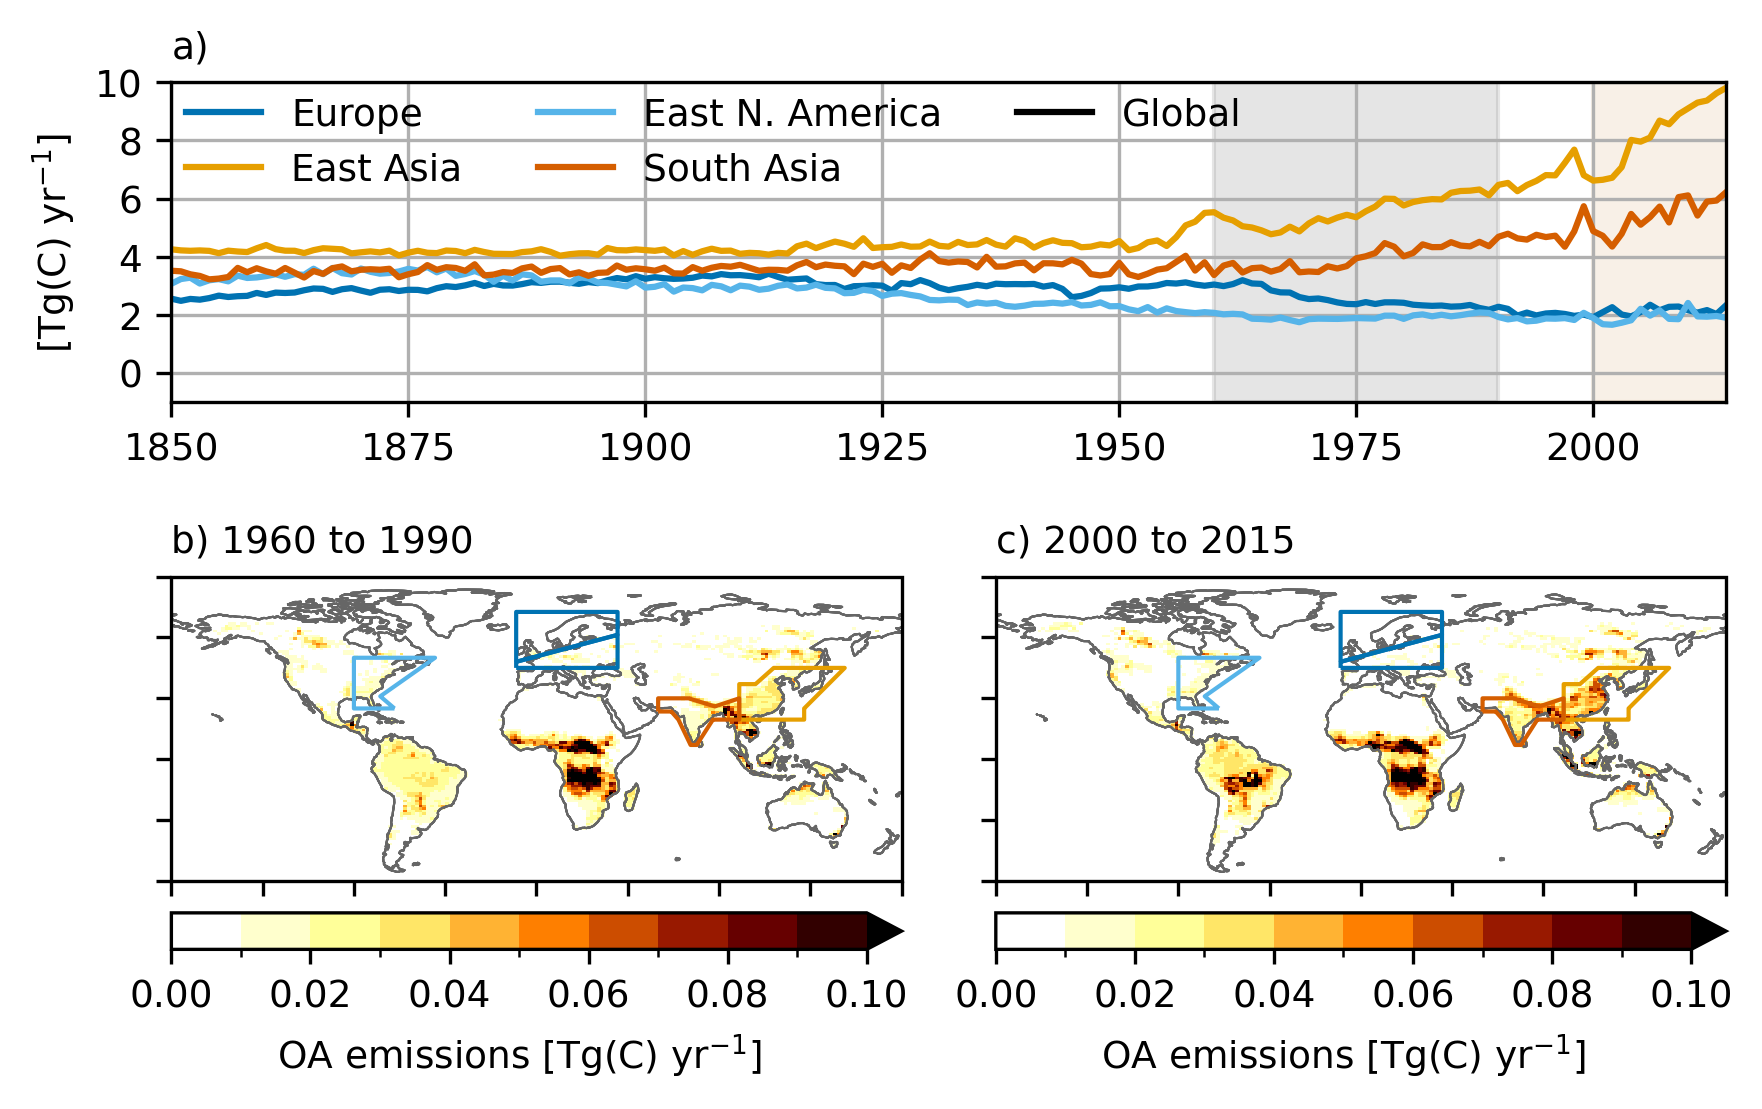
\includegraphics[width=\linewidth]{Appendix2/figs/emioa_series_histsst.png}
    \caption[Global and regional organic carbon aerosol emission trends and distribution, 1960--2015.]{a) Global and regional time series organic carbon aerosol emissions (\histsst{}). b--c) Global distribution of organic carbon aerosol emissions between 1960--1990 and 2000--2015. }
    \label{fig:app2:emioa_series}
\end{figure}

\begin{figure}[ht!]
    \centering
    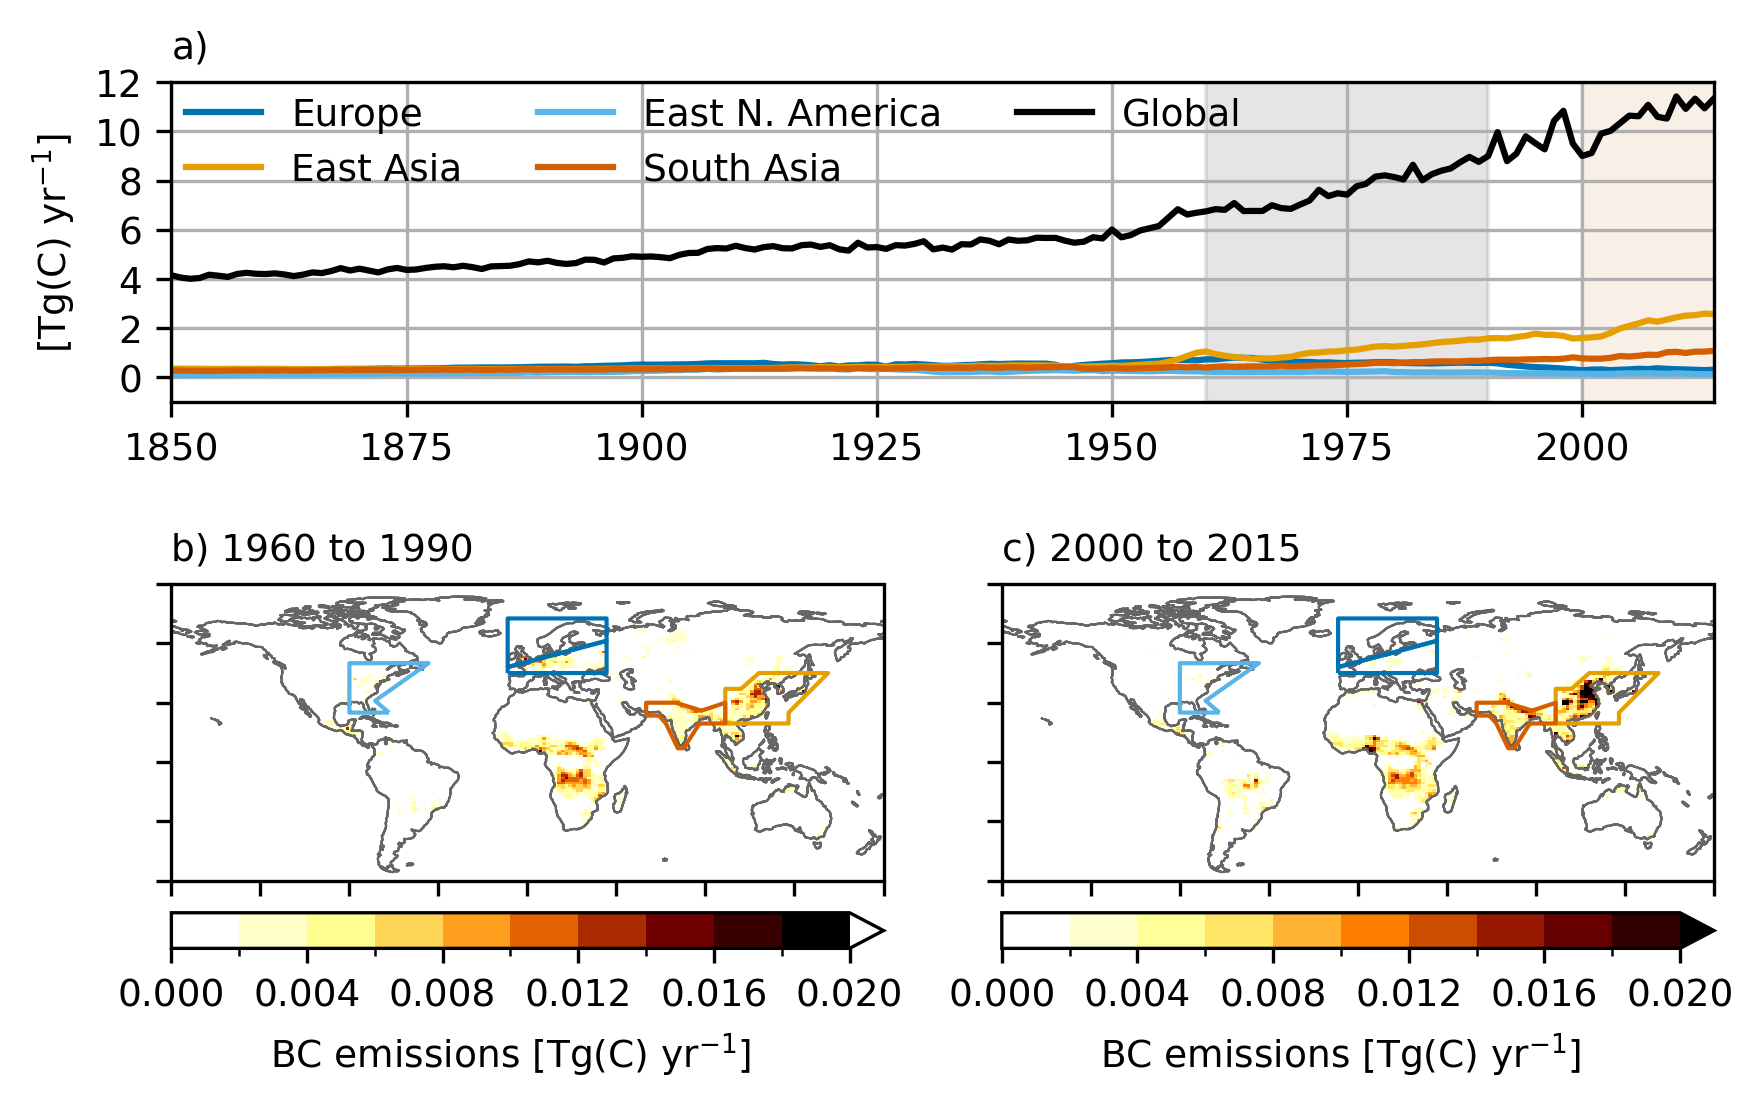
\includegraphics[width=\linewidth]{Appendix2/figs/emibc_series_histsst.png}
    \caption[Global and regional black carbon aerosol emission trends and distribution, 1960--2015.]{a) Global and regional time series of black carbon aerosol emissions (\histsst{}). b--c) Global distribution of black carbon aerosol emissions between 1960--1990 and 2000--2015. }
    \label{fig:app2:emibc_series}
\end{figure}

\begin{figure}[ht!]
    \centering
    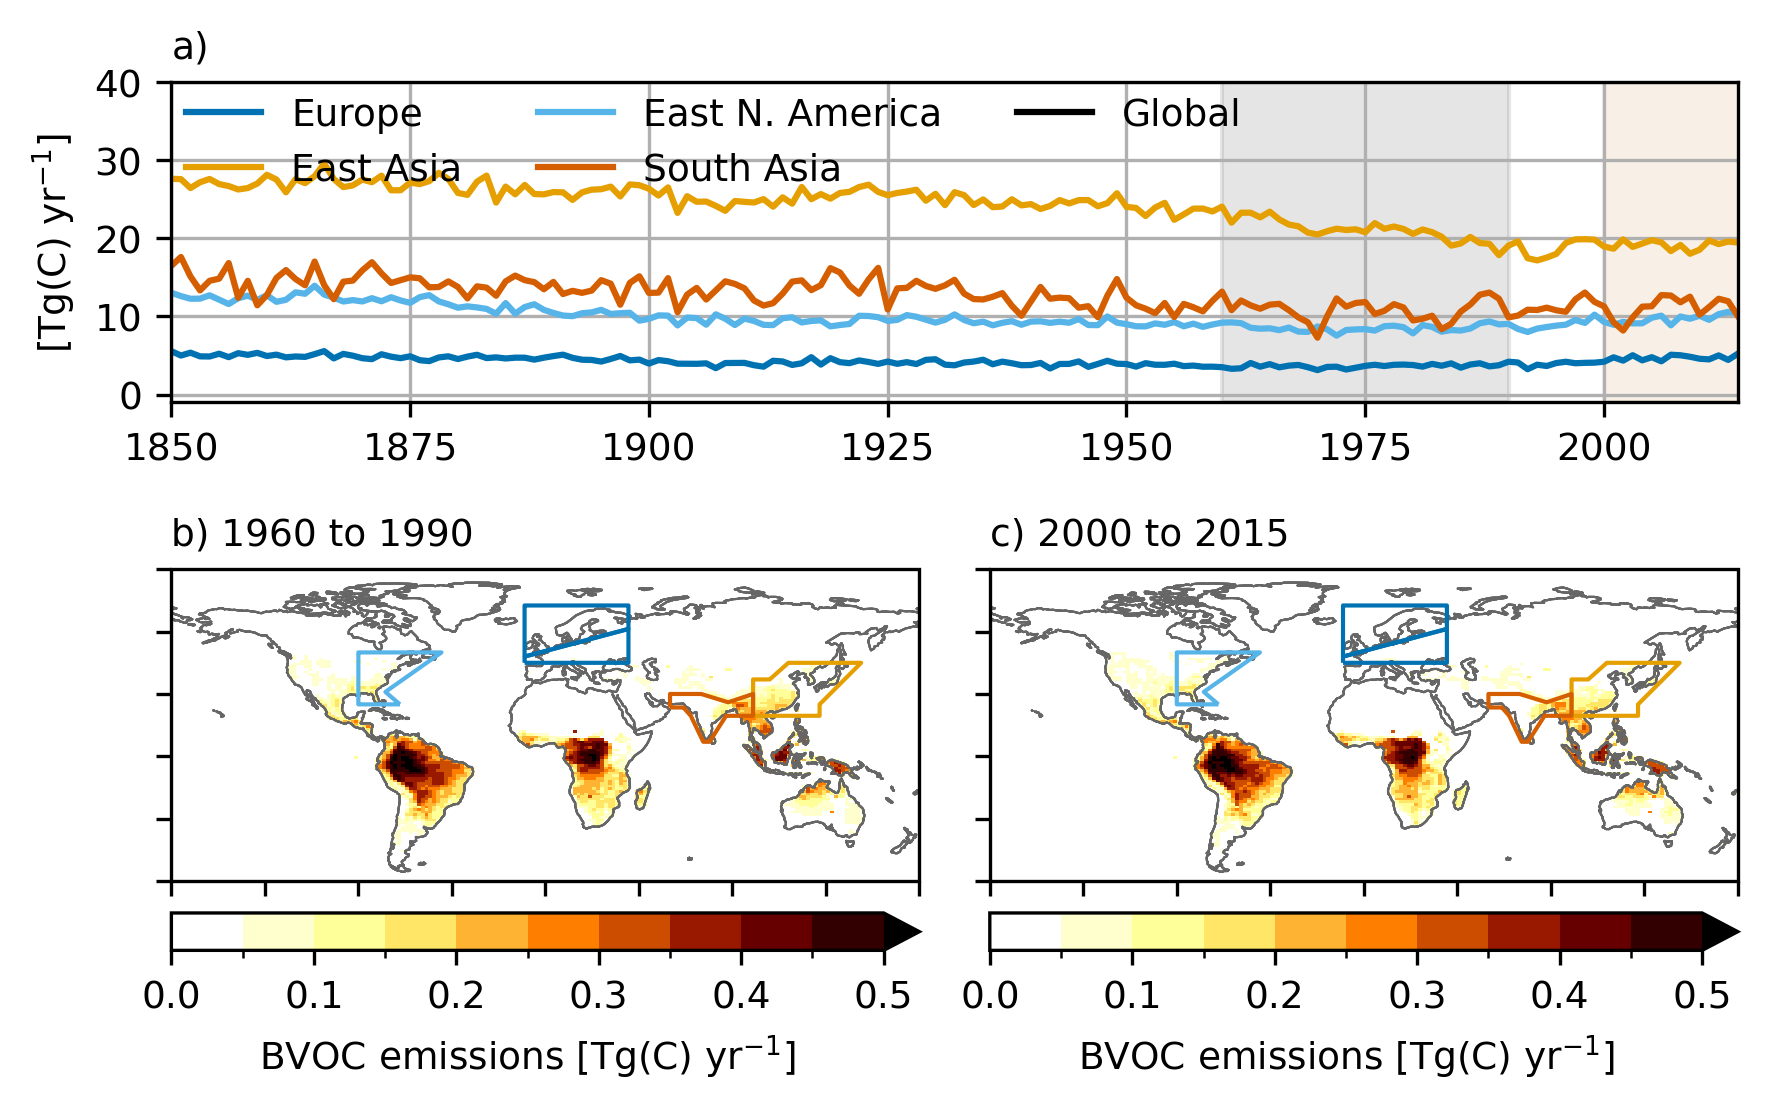
\includegraphics[width=\linewidth]{Appendix2/figs/emibvoc_series_histsst.png}
    \caption[Global and regional BVOC emission trends and distribution, 1960--2015.]{a) Global and regional time series of biogenic volatile organic compound (BVOC) emissions (\histsst{}). b-c) Global distribution of BVOC emissions between 1960--1990 and 2000--2015.}
    \label{fig:app2:emibvoc_series}
\end{figure}


\begin{figure}[ht!]
    \centering
    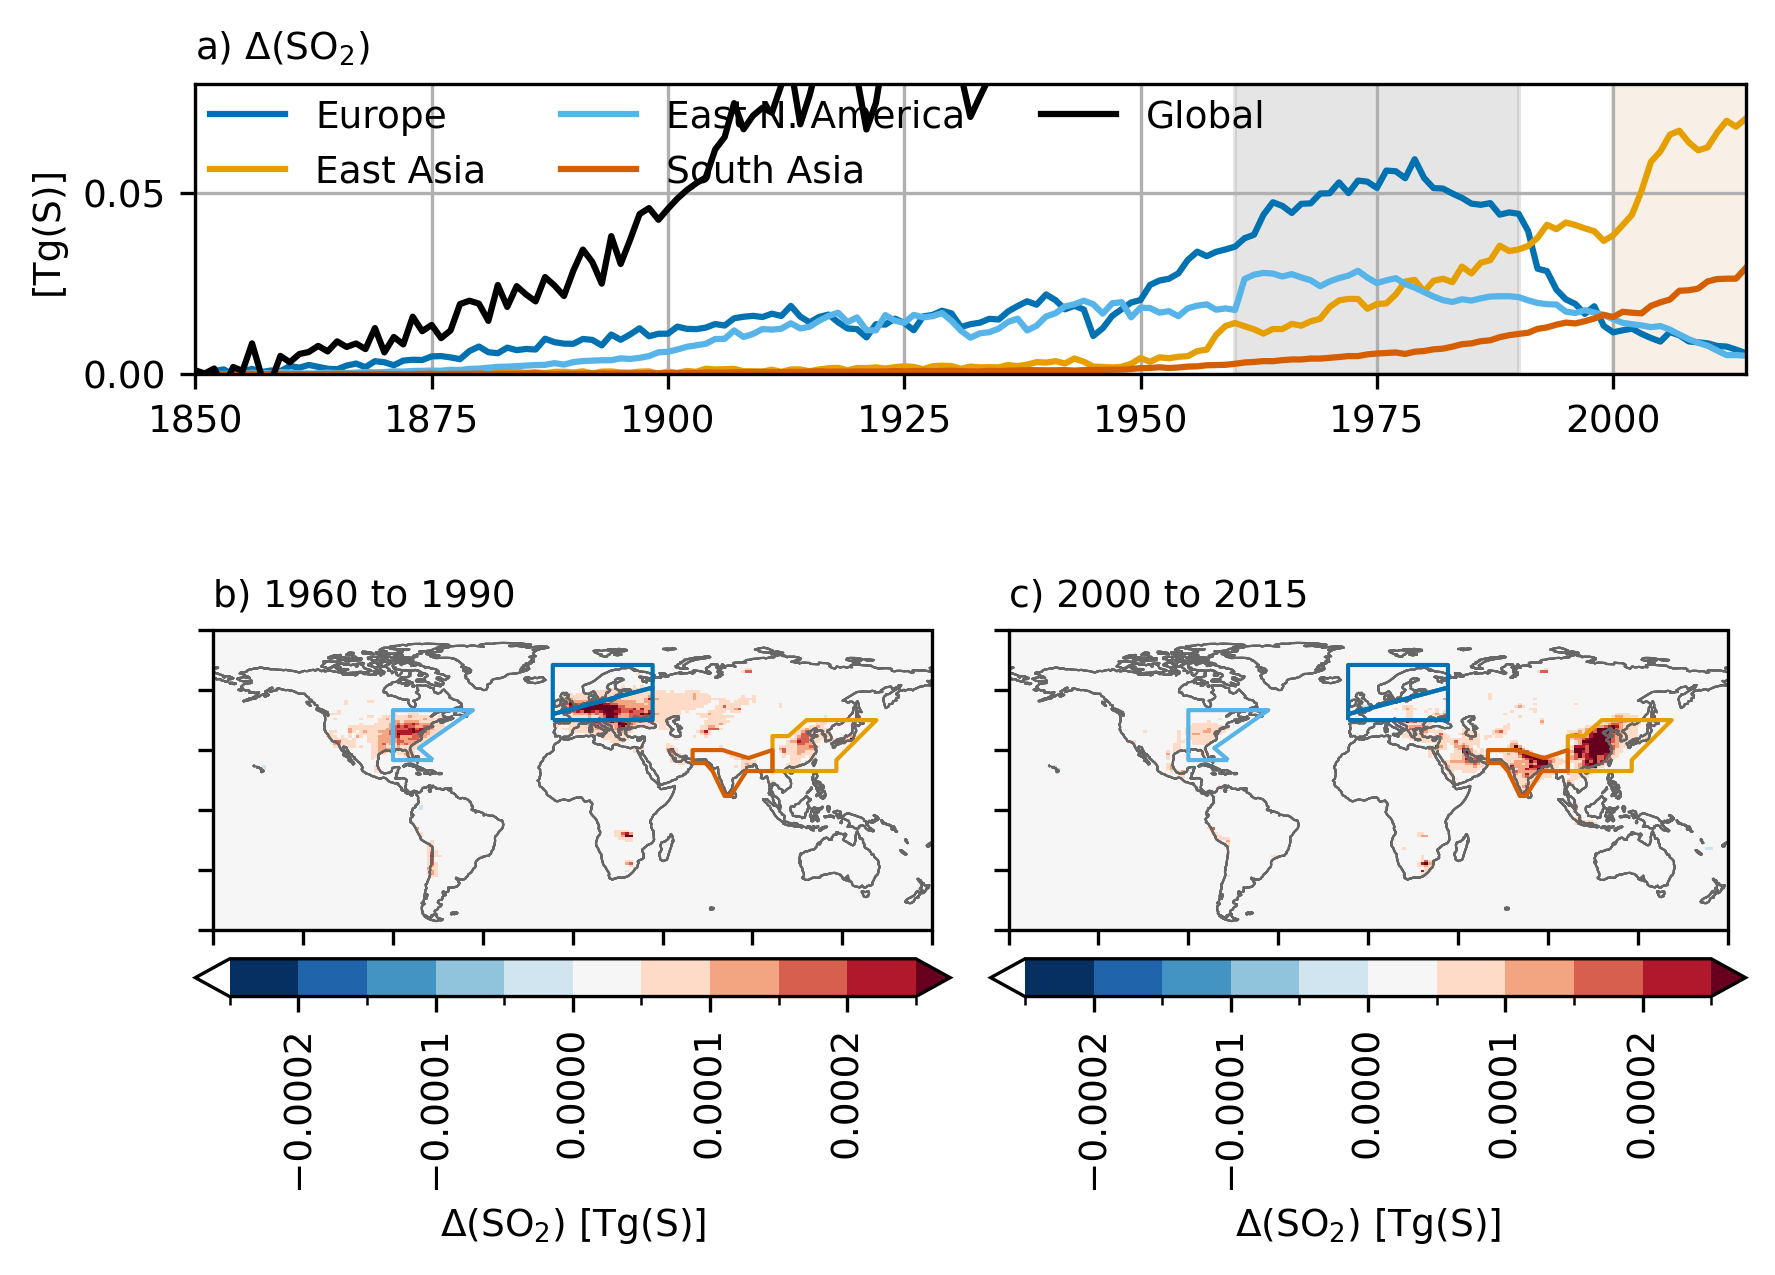
\includegraphics[width=\linewidth]{Chapter5/Figs/regional_so2_series_histsst_sstpiaer.png}
    \caption[Global and regional \ce{SO2} burden changes due to aerosol precursor emissions, 1960--2015.]{a) Global and regional time series of changes in total \ce{SO2} burden due to aerosol precursor emissions (\histsst{} minus \sstpiaer{}). b--c) Global distribution of changes in total \ce{SO2} burden due to aerosol precursor emissions between 1960--1990 and 2000--2015. }
    \label{fig:app2:so2_series}
\end{figure}


\begin{figure}[ht!]
    \centering
    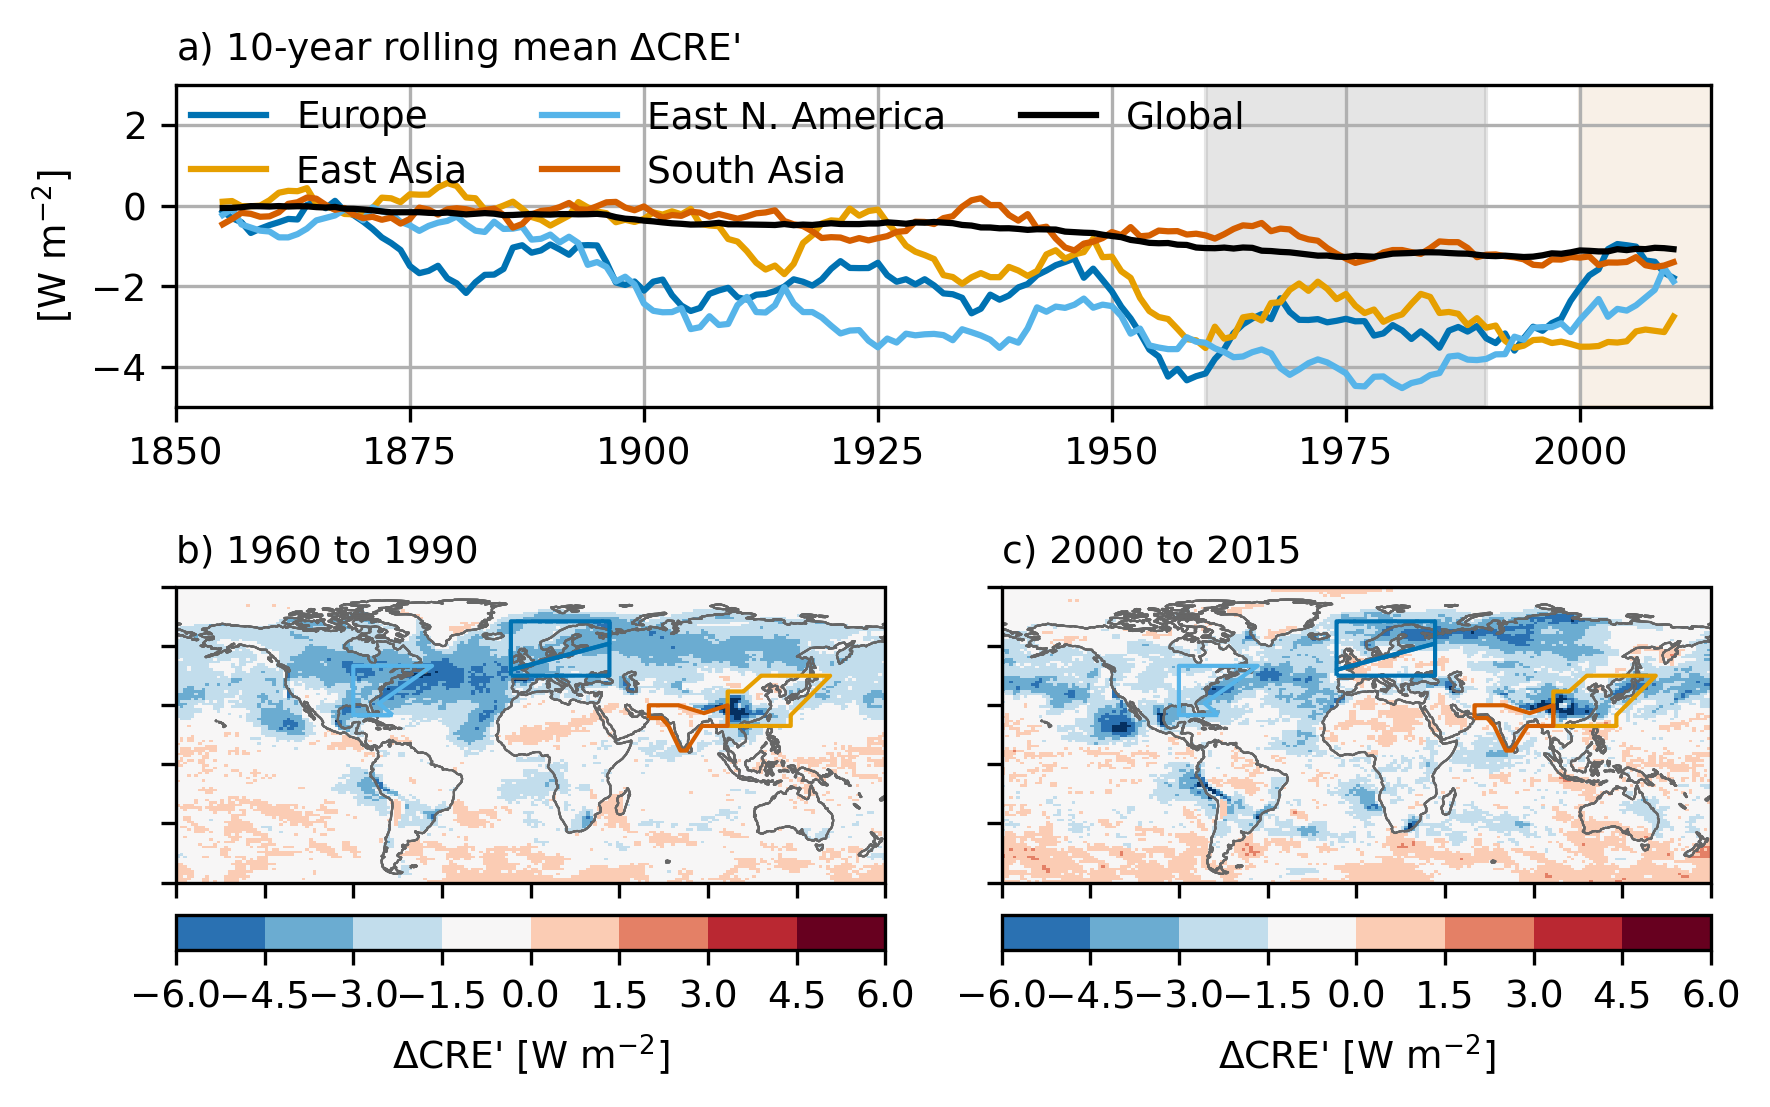
\includegraphics[width=\linewidth]{Chapter5/Figs/regional_net_toa_cloudy_series_histsst_sstpiaer.png}
    \caption[Global and regional $CRE'$ changes due to aerosol precursor emissions, 1960--2015.]{a) Global and regional time series of changes in cloud radiative effects ($CRE'$), calculated from the cloudy part of the radiative balance, due to aerosol precursor emissions (\histsst{} minus \sstpiaer{}). b--c) Global distribution of changes in $CRE'$ due to aerosol precursor emissions between 1960--1990 and 2000--2015.}
    \label{fig:ch5:cre_series}
\end{figure}

\begin{figure}[ht!]
    \centering
    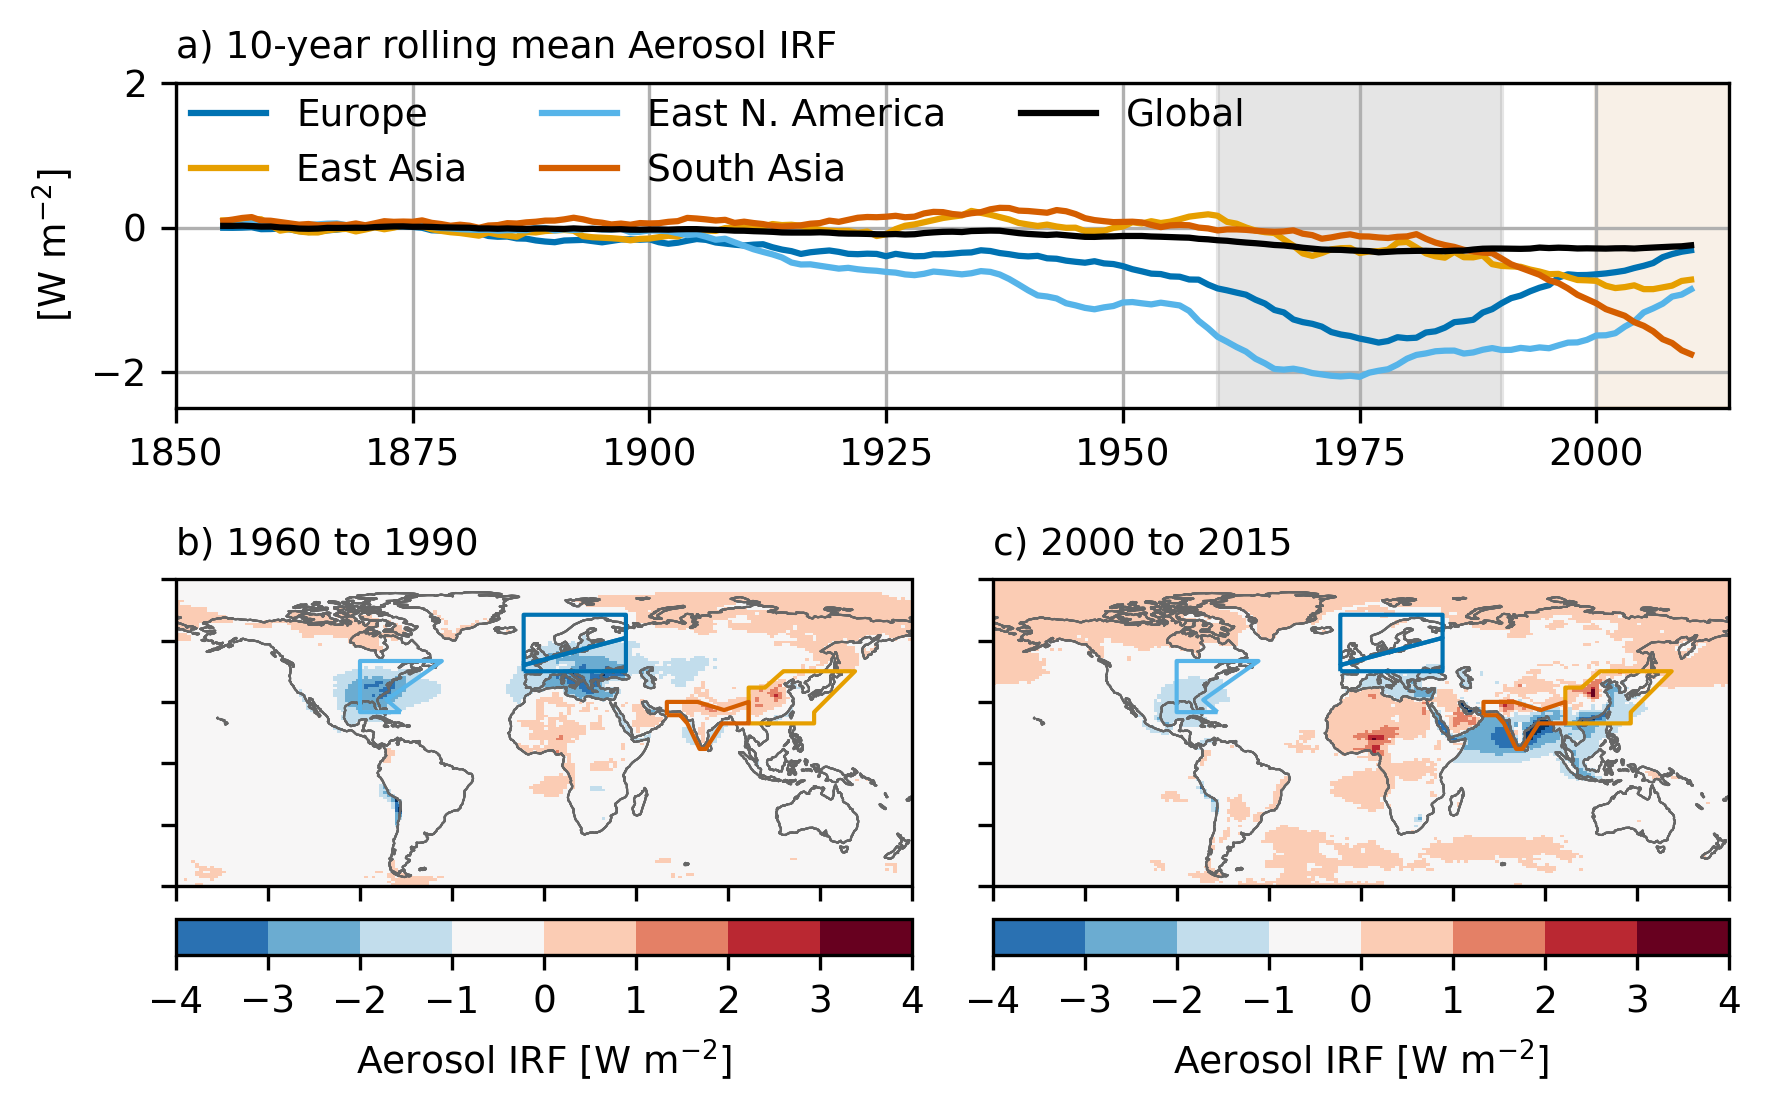
\includegraphics[width=\linewidth]{Chapter5/Figs/regional_net_toa_hazy_series_histsst_sstpiaer.png}
    \caption[Global and regional aerosol IRF changes due to aerosol precursor emissions, 1960--2015.]{a) Global and regional time series of changes in aerosol instantaneous radiative forcing (Aerosol IRF), calculated from the hazy part of the radiative balance, due to aerosol precursor emissions (\histsst{} minus \sstpiaer{}). b--c) Global distribution of changes in aerosol IRF due to aerosol precursor emissions between 1960--1990 and 2000--2015.}
    \label{fig:ch5:irf_series}
\end{figure}


\begin{figure}[th!]
    \centering
    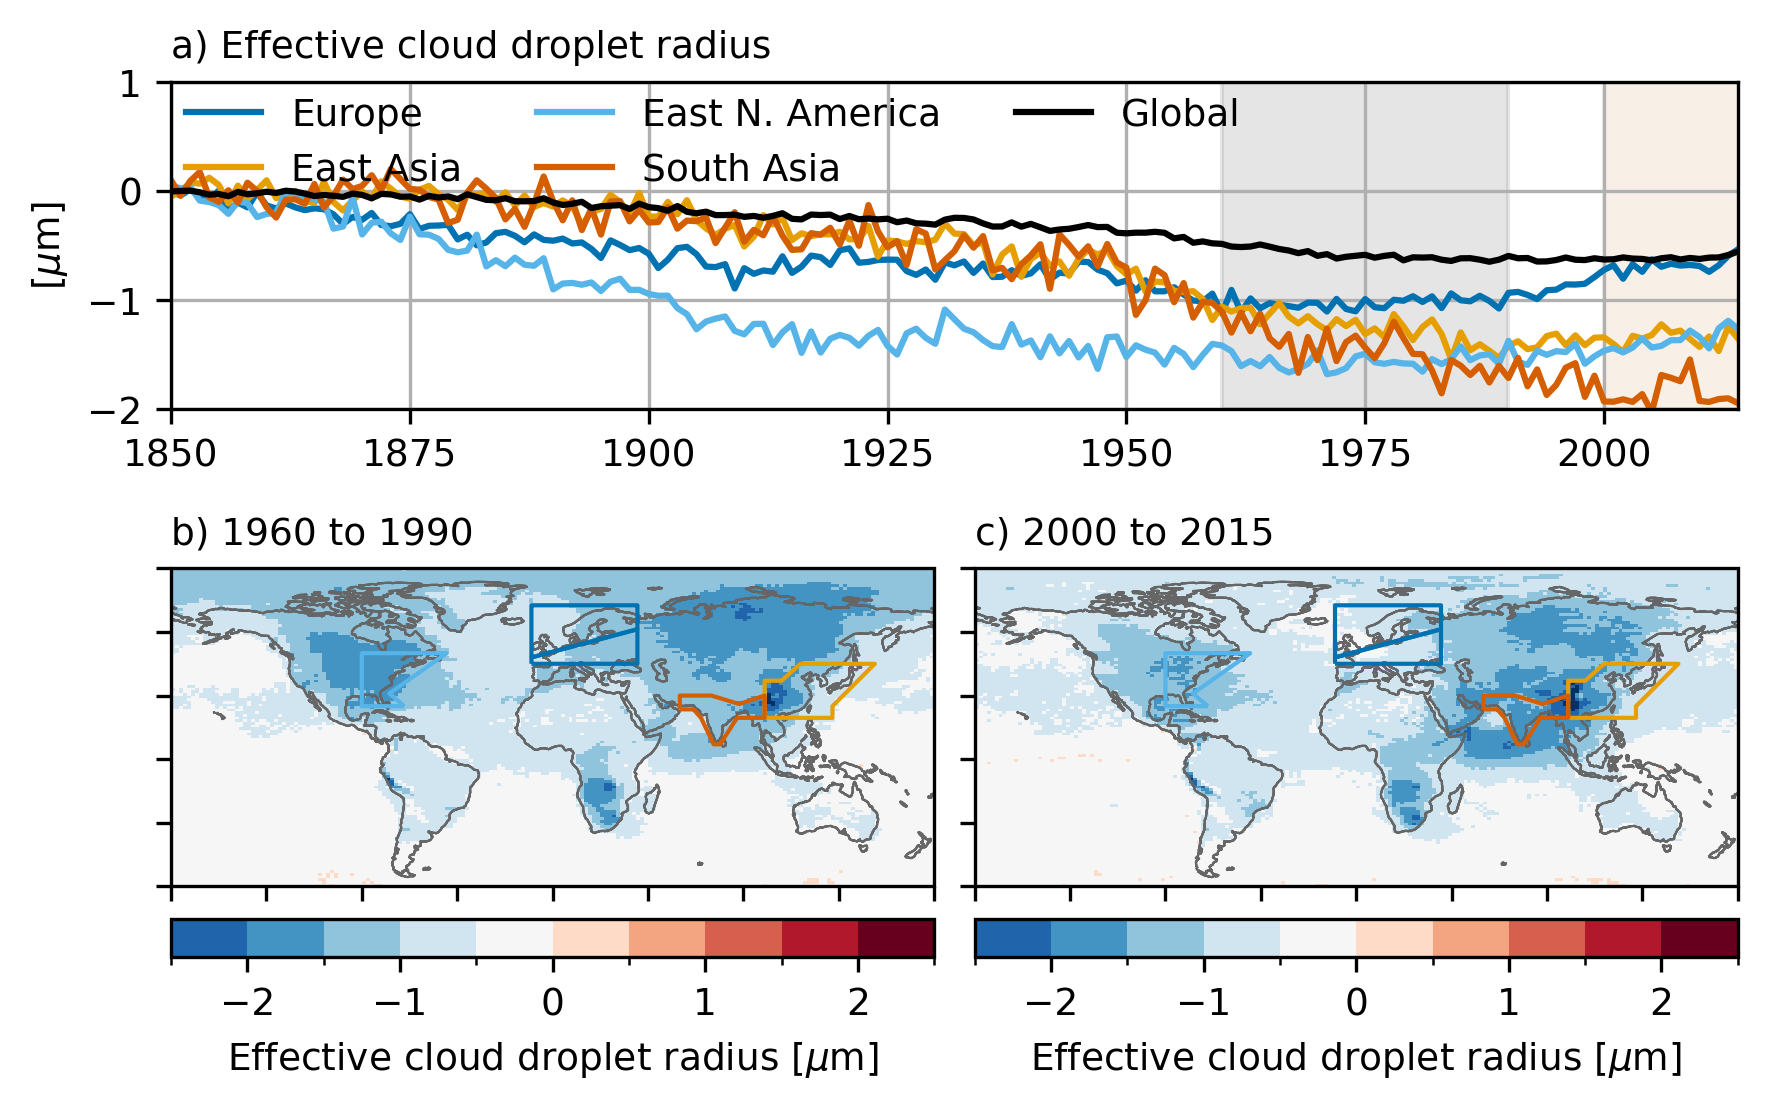
\includegraphics[width=\linewidth]{Chapter5/Figs/regional_Reff_series_histsst_sstpiaer.png}
    \caption[Global and regional \Reff{} changes (surface to 10 km) due to aerosol precursor emissions, 1960--2015.]{a) Global and regional time series of changes in effective cloud droplet radius (\Reff{}) due to aerosol precursor emissions (\histsst{} minus \sstpiaer{}) from surface to 10 km altitude. b--c) Global distribution of changes in \Reff{} due to aerosol precursor emissions between 1960--1990 and 2000--2015.}
    \label{fig:ch5:reff_series}
\end{figure}


\begin{figure}[th!]
    \centering
    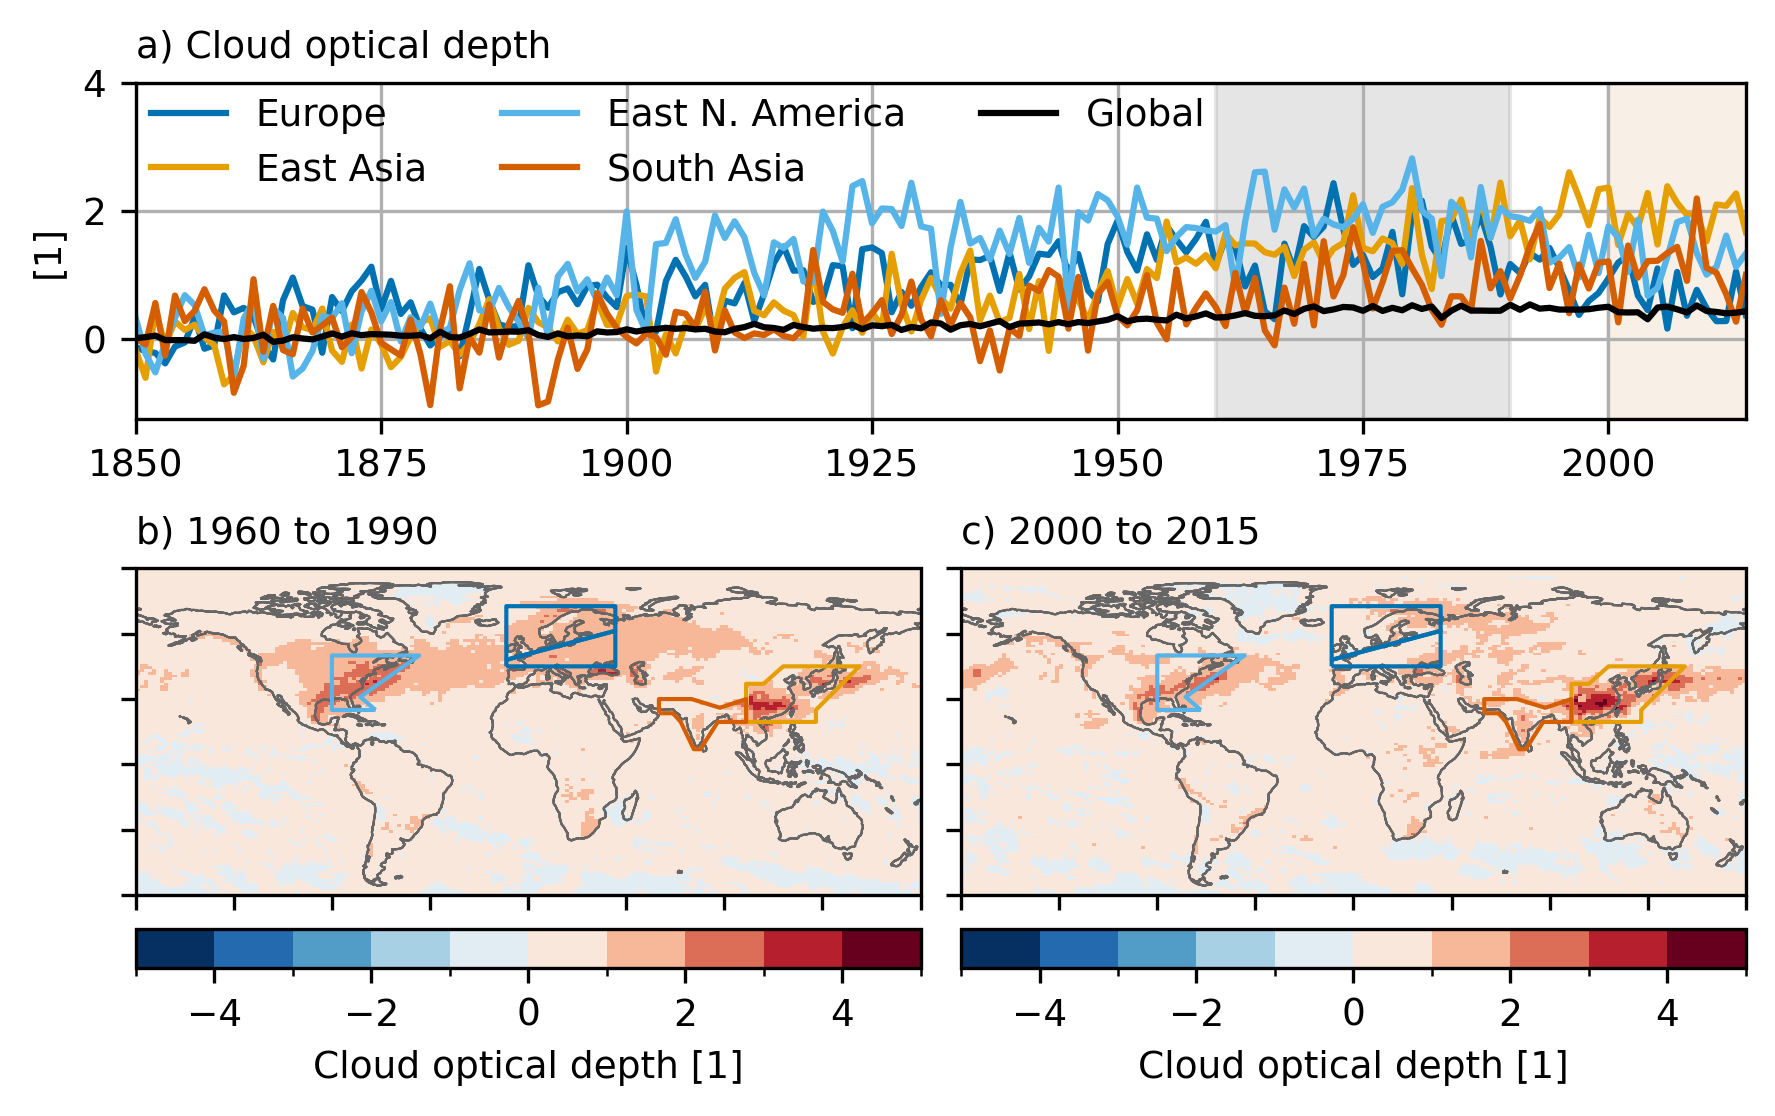
\includegraphics[width=\linewidth]{Chapter5/Figs/regional_cod_series_histsst_sstpiaer.png}
    \caption[Global and regional cloud optical depth changes due to aerosol precursor emissions, 1960--2015.]{a) Global and regional time series of changes in cloud optical depth due to aerosol precursor emissions (\histsst{} minus \sstpiaer{}). b--c) Global distribution of changes in cloud optical depth due to aerosol precursor emissions between 1960--1990 and 2000--2015.}
    \label{fig:ch5:cod_series}
\end{figure}
